% Template para la realización de la Presentacion de la Tesis.

% Tipo de Documento.
\documentclass[a4paper]{article}

% Idioma.
\usepackage[utf8x]{inputenc}
\usepackage[spanish]{babel}
\usepackage{babelbib}

% Margenes.
\usepackage[outer=4cm,inner=2cm,top=2cm,bottom=2cm]{geometry}
\usepackage{fancyhdr}
\usepackage{lastpage}

% Graficos.
\usepackage{graphicx}
\graphicspath{{./images/}}

% Codigo Fuente.
\usepackage{tabularx}

% Hypervinculos.
\usepackage{url}
\usepackage{color,hyperref}
\definecolor{black}{rgb}{0.0,0.0,0.0}
\definecolor{darkblue}{rgb}{0.0,0.0,0.3}
\hypersetup{colorlinks,breaklinks,
            linkcolor=black,urlcolor=darkblue,
            anchorcolor=darkblue,citecolor=darkblue}

% Guiones
\hyphenation{pro-ble-ma}
\hyphenation{ge-ne-ra-ra}
\hyphenation{pos-te-rior-men-te}

% Definicion de la hoja de firmas.
\newcommand{\signature}[7]{
	\vfill

	\begin{flushright}
		#1, \today
	\end{flushright}
	\vspace{3cm}

	\noindent
	\centering
	\begin{tabularx}{0.9\textwidth}{cXc}
		\multicolumn{3}{c}{\rule{5cm}{1pt}}\\
		\multicolumn{3}{c}{#2}\\
		\multicolumn{3}{c}{#3}\\
		\vspace{3cm}\\
		\rule{5cm}{1pt} & \hspace{2.5cm} & \rule{5cm}{1pt} \\
		#4 & ~ & #5 \\
		#6 & ~ & #7
	\end{tabularx}
	\vspace{1cm}
}

% Encabezado y Titulo del Documento y de la Tesis.
\title{
	{\normalsize
		Universidad de Buenos Aires\\
		Facultad de Ingeniería -- Departamento de Electrónica\\
		Propuesta de Tesis de Ingeniería Electrónica\\
		\vspace{0.7cm}
	}
	Diseño, validación e implementación de una microarquitectura RISC
}

% Datos de autor: Tesista, Director y Co-director.
\author{	\textbf{Tesista}															\\
			Luciano César Natale, \textit{Padrón Nro. 86.659}               			\\
            \texttt{ \href{mailto:luchonat@gmail.com}{luchonat@gmail.com}}			\\[2.5ex]
            \textbf{Director}																\\
            Ing. Nicolas Alvarez, \textit{Profesor Adjunto}             				\\
            \texttt{ \href{mailto:nalvare2001@yahoo.com.ar}{nalvare2001@yahoo.com.ar}}  \\[2.5ex]
            \textbf{Co-director}															\\
            Ing. Octavio Alpago, \textit{JTP. Interino}               					\\
            \texttt{ \href{mailto:oalpago@gmail.com}{oalpago@gmail.com}}                \\[2.5ex]
       }

% Fecha.
\date{\today}

% Pie de Pagina.
\pagestyle{fancy}
\lhead{}
\chead{}
\rhead{}
\lfoot{}
\cfoot{
	{\footnotesize
	\emph{Diseño, validación e implementación de una microarquitectura RISC}\\
	Plan de Tesis -- Página \thepage\ de \pageref{LastPage}
	}
}
\rfoot{}
\renewcommand{\headrulewidth}{0pt}
\renewcommand{\footrulewidth}{0.4pt}

% Documento.
\begin{document}

\maketitle

%\thispagestyle{empty}

%\begin{abstract}
%\end{abstract}

\thispagestyle{fancy}

\section{Objeto y área de la tesis}

El objetivo principal de este trabajo consiste en diseñar, validar e implementar una microarquitectura RISC\footnote{\label{RISC}: Reduced instruction set computer. Técnica de diseño de unidades de procesamiento basadas en el hecho de que un conjunto de instrucciones simples provee una mayor performance al ser combinado con una microarquitectura capaz de ejecutar dichas instrucciones en algunos pocos ciclos de máquina.}. El diseño incluirá la completa especificación funcional de la microarquitectura y su conjunto de instrucciones (¿agregar algo de que soporta instrucciones CORDIC?). El diseño se validará mediante el desarrollo en software de un emulador de la arquitectura; la implementación se realizará en el lenguaje de descripción de hardware Verilog, y se sintetizárá en un dispositivo FPGA\footnote{\label{FPGA}Field Programmable Gate Array: dispositivo semiconductor que contiene bloques de lógica cuya interconexión y funcionalidad puede ser configurada `in situ' mediante un lenguaje de descripción especializado.}.

El interés en este desarrollo proviene de la necesidad de contar con un núcleo de procesamiento altamente configurable y suficientemente flexible y sencillo para distintas aplicaciones dentro del ámbito de la investigación en los laboratorios de microelectrónica (¿y de sistemas embebidos?); sintetizable en FPGA
(¿y en silicio?).

El área profesional de relevancia del trabajo de tesis es el diseño de sistemas digitales y su aplicación como base de proyectos de investigación que necesiten de un núcleo de procesamiento configurable y sencillo.

\newpage

\section{Introducción, antecedentes y actualidad}

Desde la aparición de los microprocesadores a mediados de los años 70, la tendencia fue el aumento de la complejidad de las arquitecturas, generando un efecto de ``bola de nieve'', al ir superponiendo capas sobre un núcleo central. Existió, entonces, una reacción adversa a esta tendencia. Por ejemplo, la arquitectura experimental de IBM 801; y también en Berkeley, David Patterson y Ditzel fueron los primeros en acuñar el término RISC, para descibir una nueva clase de microarquitectura que deshacía el camino del resto de las arquitecturas hasta el momento, conocidas, en contraposición, como CISC\footnote{\label{CISC}: Complex instruction set computer. Técnica de diseño de unidades de procesamiento basadas en el hecho de que el conjunto de instrucciones debe ser lo más poderoso posible.}. A partir de este antecedente, los principales fabricantes de microprocesadores han lanzado al mercado sus propias implementaciones basadas en los principios establecidos en IBM y Berkeley.

El concepto de las arquitecturas RISC se basa, principalmente, en el hecho de que al simplificar la lógica necesaria para la ejecución de una instrucción, permite aumentar la frecuencia de operación de las compuertas que componen la lógica. Además, es posible dividir la ejecución de las instrucciones en etapas sencillas y consecutivas, permitiendo de esta manera implementar fácilmente optimizaciones como, por ejemplo, una arquitectura de \emph{pipeline}\footnote{\label{Pipeline}: Técnica de diseño...}. Es por eso que el conjunto de instrucciones es sencillo, permitiendo solamente operaciones básicas entre registros internos del microprocesador. El trabajo realizado por cada instrucción, en general, es menor que el generado por una instrucción CISC, pero se hace de manera sencilla y rápida. Es importante notar que no solamente la ganancia radica en poder aumentar la frecuencia de operación de la lógica, sino que estas condiciones facilitan el desarrollo de diseños de bajo consumo, característica muy valorada en el nicho de los sistemas embebidos.

El mercado de los sistemas embebidos es excesivamente amplio y está inserto en todas las industrias. En un automóvil, por ejemplo, podemos encontrar microprocesadores, en el sistema de frenos, en la central de inyección electrónica, en el sistema de entretenimiento y navegación, etc. La otra arista de vital importancia para el mercado de los sistemas embebidos, es el de los dispositivos móviles, donde se vuelve vital el requerimiento de bajo consumo. Estamos viviendo la revolución de IoT\footnote{\label{Internet of Things} Definición... }, que se trata básicamente de sistemas embebidos autónomos que estan conectados a ``la nube'' y pueden ser monitoreados y controlados remotamente a través de \emph{Internet}.

Dentro del universo de las arquitecturas RISC, actualmente destacan dos: MIPS y ARM. La primera, fue desarrollada por un grupo de investigadores de la Universidad de Stanford (entre ellos John L. Hennessy, pionero del concepto RISC junto a David Patterson, coautores de la bibliografía más relevante del área). Esta arquitectura, por su sencillez, es la predilecta al momento del desarrollo de cursos enfocados en la enseñanza de arquitectura de computadoras. Si bien esta arquitectura posee gran relevancia académica, es muy popular en el mercado de los microprocesadores en sistemas embebidos como equipos de telecomunicaciones, decodificadores de TV digital, y consolas de entretenimiento con ejemplos muy conocidos como \emph{Nintendo} y \emph{PlaySation}. ARM, por otro lado, ha ganado una importante porción del mercado de los embebidos (con un gran aporte de los dispositivos móviles), basando su modelo de negocios en la venta de la propiedad intelectual del diseño de los microprocesadores a las empresas que finalmente producen el silicio.

\section{Desarrollo previsto de la tesis}

\subsection{Teoría, enfoque y métodos a utilizar}

El enfoque de la tesis se basará en un desarrollo teórico del conjunto de instrucciones y de las características de la microarquitectura; y en el desarrollo
práctico del emulador y la implementación en lenguaje descriptor de hardware.

El concepto central detrás del desarollo será el de \textbf{ortogonalidad}, en el sentido de que cada bloque constructivo de la arquitectura sea independiente e indiferenciable del resto de la arquitectura, llevando así al extremo la sencillez del diseño.

Acá me falta....

\subsection{Estudios conexos}

Asignaturas y otros estudios ¿previstos o previos? que son relevantes al desarrollo de la tesis.

\begin{itemize}
	\item \textbf{Sistemas digitales:} asignatura que abarca la teoría de técnicas de diseño de hardware digital y codificación de sistemas digitales, así como también su síntesis y medición.
	\item \textbf{Organización de computadoras:} asignatura en la cual se cubren los aspectos teóricos del diseño de microarquitecturas.
	%\item \textbf{Procesamiento de Señales:} Asignatura que abarca los conceptos respecto al procesamiento de señales y el uso de filtros adaptativos.
\end{itemize}

\subsection{Alcance proyectado para la tesis}

Como resultados a obtener de la tesis se tienen los siguientes:

\begin{itemize}
    \item Especificación completa de la microarquitectura
    \item Vectores de prueba
    \item Emulador de la arquitectura
    \item \emph{IP Core} codificado en el lenguaje \emph{Verilog} de la microarquitectura completa
    \item Resultado de los vectores de prueba tanto en el emulador como en el \emph{IP Core}
    \item Análisis comparativo entre la microarquitectura desarrollada y otras arquitecturas RISC
    \item Proposición de trabajos futuros y/o mejoras.
\end{itemize}

Para asegurar que el proyecto de tesis incluya todos los trabajos requeridos, los procesos a completar se describen en un plan de trabajo en la siguiente sección.

\newpage

\subsection{Plan de trabajo}

%Planificación y definición: descomponer la totalidad de la tesis en las tareas, procesos y fases, necesarios para lograr el resultado. Indicar cómo se definirá, verificará y controlará el alcance previsto de la tesis. Incluir un plan de trabajo tentativo, estimando los plazos de ejecución de cada parte.

La duración total del trabajo se estima en un año y se considera que la misma estará compuesta por las siguientes etapas:

\begin{itemize}
    \item \textbf{Investigación bibliográfica:} recolección de libros, \emph{papers}, trabajos de tesis, y fuentes de investigación con el objetivo de obtener el entendimiento teórico requerido y conocer el estado del arte en el tema a trabajar.
    \item \textbf{Introducción al trabajo de tesis:} comprender la teoría de las microarquitecturas RISC. Describir el contenido teórico requerido para exponer los conceptos de funcionamiento del hardware a desarrollar.
    \item \textbf{Análisis de arquitecturas existentes:} analizar las diferentes arquitecturas existentes con sus pro y contras. Obtener de este análisis las relaciones de compromiso asumidas en ellas para poder aplicarlas en la arquitectura a desarrollar.
    \item \textbf{Diseño de la microarquitectura y su conjunto de instrucciones:} realizar la especificación funcional de la microarquitectura y su conjunto de instrucciones.
    \item \textbf{Validación:} desarrollar los vectores de pruebas que permitirán validar la microarquitectura.
    \item \textbf{Emulación:} desarrollar el emulador de la microarquitectura y validar los vectores de pruebas.
    \item \textbf{Implementación:} desarrollar el \emph{IP core} en un ambiente de simulación y, en la medida que sea posible, en campo. Realizar la síntesis de la misma para distintos dispositivos FPGA, medir recursos utilizados, máxima frecuencia de operación y potencia consumida. Validar los vectores de pruebas.
    \item \textbf{Conclusiones y trabajos a futuro:} se extraerán las conclusiones pertinentes sobre los resultados obtenidos y se propondrán, si correspondiese, futuras mejoras de la microarquitectura.
    \item \textbf{Preparación del informe final:} se consolidará la documentación con la memoria de la tesis la cual contendrá el resultado de todo el trabajo realizado. Se revisará la tesis por el Director, Co-director y por los pares antes de enviarla al Jurado.
    \item \textbf{Preparación de la presentación y defensa de la tesis:} se elaborarán diapositivas para la presentación con los objetivos, alcance, introducción a las microarquitecturas RISC, desarrollo de la microarquitectura, resultados obtenidos, conclusiones y trabajos a futuro. La misma será posteriormente utilizada para la defensa.
\end{itemize}

En la figura \ref{TablaActividades} se encuentra el plan propuesto para la formación del tesista y el cumplimiento de los objetivos.

\begin{figure}[h!]
	\label{TablaActividades}
	%trim option's parameter order: left bottom right top
	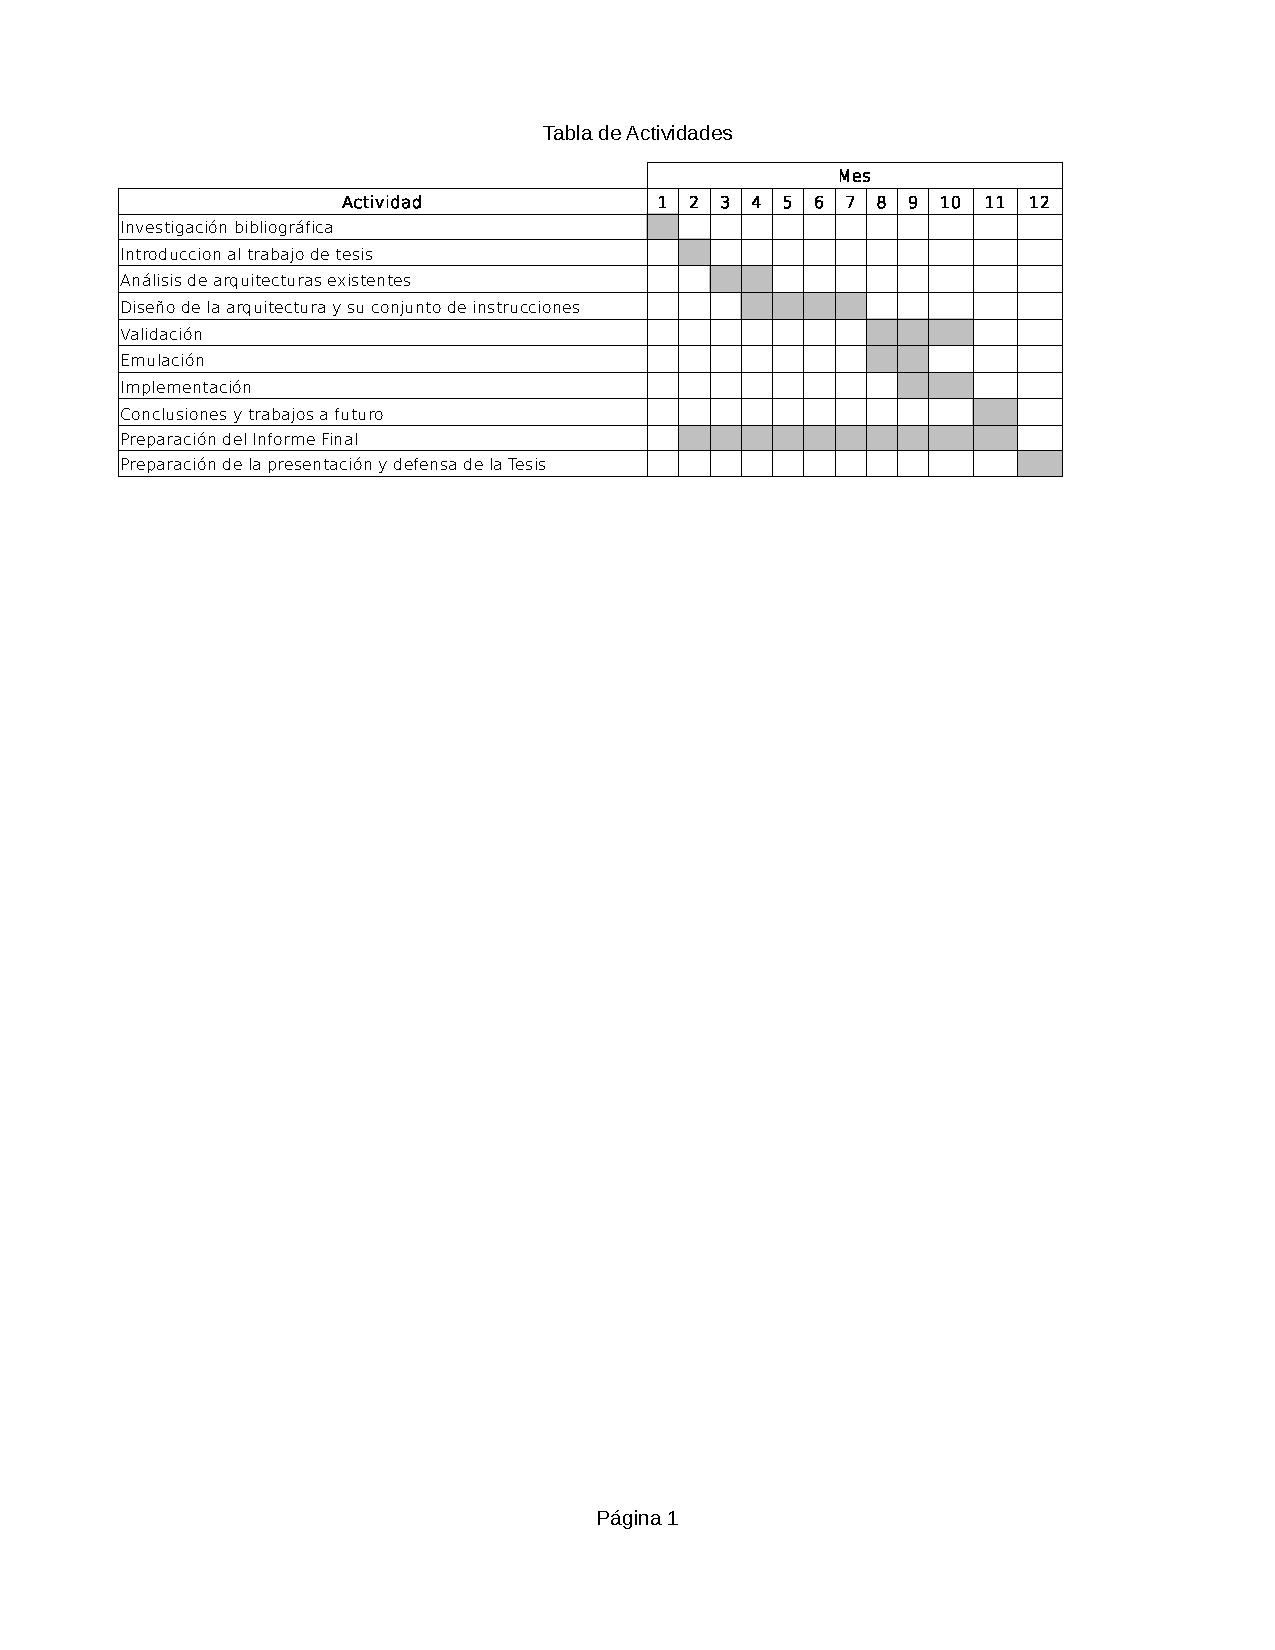
\includegraphics[trim = 20mm 200mm 20mm 25mm, clip, width=\textwidth]{tabla_actividades}
	\caption{Diagrama de las actividades a realizar por el tesista.}
\end{figure}

\newpage

\section{Bibliografía}

CAMBIARLA!!!

\begin{thebibliography}{99}

\bibitem{Mohammadi} Abbas Mohammadi \& Fadhel M. Ghannouchi, ``RF Transceiver Design for MIMO Wireless Communications'', Springer, p1-5, 2012.
\bibitem{Paulraj} Paulraj, A., Nabar, R., Gore, D., ``Introduction to Space-Time Wireless Communications''. Cambridge University Press, 2003.
\bibitem{Litva} John Litva \& Titus Kwok-Yeung Lo, ``Digital Beamforming in Wireless Communications'', Artech House, 1996.
\bibitem{Mohammadi2} Abbas Mohammadi \& Fadhel M. Ghannouchi, ``RF Transceiver Design for MIMO Wireless Communications'', Springer, p17-20, 2012.
\end{thebibliography}

\newpage

\signature{Buenos Aires}{Sr. Luciano César Natale}{Tesista}{Ing. Nicolás Alvarez}{Ing. Octavio Alpago}{Prof. Adjunto, Director}{JTP. Interino, Co-director}

\end{document}
